% =============================================================================
% Phase I report - SIMD Vector Processing Unit
% Build:  make report   (or: cd reports/src && tectonic -X compile main.tex)
% =============================================================================
\documentclass[conference]{IEEEtran}
\usepackage[T1]{fontenc}
\usepackage{graphicx}
\usepackage{booktabs}
\usepackage{amsmath}
\usepackage{siunitx}
\usepackage{url}
\usepackage{xcolor}
\usepackage{listings}
\usepackage[hidelinks]{hyperref}

% ---- Edit these two lines with the official affiliation ---------------------
\newcommand{\AFFIL}{Department of Computer Applications}
\newcommand{\INST}{University Name, City, India}

\lstset{basicstyle=\ttfamily\footnotesize, columns=fullflexible, frame=single,
        framerule=0.3pt, rulecolor=\color{gray}, xleftmargin=2pt, xrightmargin=2pt,
        commentstyle=\color{gray}, morecomment=[l]{\#}}

\begin{document}

\title{Design and Evaluation of a Parameterised\\SIMD Vector Processing Unit on FPGA}

\author{
\IEEEauthorblockN{Mahir\IEEEauthorrefmark{1}, Krishiv Gupta\IEEEauthorrefmark{1}, Abhiman Singh\IEEEauthorrefmark{1}, Jayadeep\IEEEauthorrefmark{1} and Ashish Kushwaha\IEEEauthorrefmark{1}}
\IEEEauthorblockA{\IEEEauthorrefmark{1}\AFFIL, \INST\\
Repository: \url{https://github.com/mahir-m01/SIMD-Vector-Processing-Unit}}
}

\maketitle

% =============================================================================
\begin{abstract}
Many workloads in signal processing, graphics and machine learning apply the same
arithmetic to long arrays of numbers. Single-instruction, multiple-data (SIMD)
hardware exploits this regularity by letting one instruction drive several
arithmetic lanes at once. This report presents the Phase~I design of a small,
fully parameterised SIMD vector processing unit written in Verilog. It provides
eight 128-bit vector registers split into eight 16-bit lanes, a 14-operation lane
ALU replicated per lane, per-lane operand multiplexers for scalar broadcast, and a
result combiner whose adder tree turns a dot-product step into one instruction.
Setting the lane count to one turns the same design into a scalar processor,
which gives a like-for-like baseline: same instruction set, same program, same
timing rules. A Python golden model, unit and system testbenches and mutation
tests verify the design. All six test programs match the model exactly in
memory, registers and cycle count for 1, 2, 4 and 8 lanes. On five benchmark
kernels, eight lanes need $7.87$--$7.92\times$ fewer clock cycles than one. After
place-and-route on a Lattice ECP5-25F, the 8-lane unit uses 19\% of the logic and
closes timing at \SI{33.6}{MHz}, against \SI{50.8}{MHz} for one lane, giving a
wall-clock speed-up of $5.2\times$.
\end{abstract}

\begin{IEEEkeywords}
SIMD, vector processor, data-level parallelism, FPGA, Verilog, hardware verification.
\end{IEEEkeywords}

% =============================================================================
\section{Introduction}

A scalar processor spends most of its effort on control: fetching, decoding and
sequencing each instruction. When a program adds two arrays, that effort is
repeated for every element, although every element needs the same work. A SIMD
processor issues one instruction for a group of elements. The control cost is paid
once and the arithmetic is replicated across \emph{lanes}. This is
\emph{data-level parallelism}, the form of parallelism behind vector
supercomputers, multimedia instruction-set extensions and GPUs~\cite{hp6}.

The goal of this project is to design such a unit at a scale that can be built,
verified and measured within a semester, and to answer three questions with
numbers rather than claims:
\begin{enumerate}
\item How close to the ideal $N\times$ does an $N$-lane unit come, measured in clock cycles?
\item What does each extra lane cost in FPGA logic, multipliers and memory?
\item How much does the wider datapath slow the clock, and what wall-clock speed-up is left?
\end{enumerate}

The Phase~I contributions are:
\begin{itemize}
\item a synthesizable, lane-parameterised SIMD unit in Verilog with the blocks named
      in the project brief: vector register file, parallel ALUs, vector control unit,
      lane multiplexers, result combiner and a scalar interface (Section~\ref{sec:design});
\item a 48-instruction ISA (14 ALU operations in three forms plus six
      others), an assembler and an instruction-level golden model that
      predicts results and exact cycle counts (Section~\ref{sec:isa});
\item a layered verification flow with self-checking testbenches, coverage counters
      and mutation tests (Section~\ref{sec:verif});
\item a scalar-versus-SIMD comparison on five kernels and an FPGA resource and
      frequency sweep over 1, 2, 4 and 8 lanes (Section~\ref{sec:results}).
\end{itemize}

% =============================================================================
\section{Literature Review}

\subsection{Taxonomy and early vector machines}
Flynn's taxonomy~\cite{flynn72} classifies machines by the number of instruction
and data streams. SIMD names the case of one instruction stream acting on many data
elements. The first commercially successful SIMD designs were vector supercomputers
such as the Cray-1~\cite{cray1}. Its vector registers and pipelined functional units
let one instruction process up to 64 elements, which hid memory latency and avoided
the instruction-issue cost of a scalar loop. Hennessy and Patterson~\cite{hp6} trace
the same principles from vector machines to subword-SIMD extensions and GPUs.

\subsection{Subword SIMD in general-purpose processors}
Intel MMX~\cite{mmx} introduced \emph{packed} data types: one 64-bit register
treated as eight bytes or four 16-bit words, with one instruction operating on all
of them. Streaming SIMD Extensions (SSE)~\cite{sse} widened the registers to 128
bits. ARM NEON uses the same width. Two conventions from this line of work are
adopted here directly: compare instructions that write all-ones or all-zeros masks,
so conditionals need no branch, and a fixed 128-bit register divided into lanes.

\subsection{Scalable vector architectures}
VIRAM~\cite{viram} showed that a vector architecture with lanes scales across
embedded media workloads more simply than superscalar or VLIW designs. A compiler
could vectorise most kernels automatically. Asanovi\'c~\cite{asanovic98} analysed
lane-based vector microprocessors in depth. Lee~\emph{et al.}~\cite{maven} compared
MIMD, vector-SIMD, subword-SIMD and SIMT designs and found vector cores more
efficient even on fairly irregular kernels. The RISC-V vector extension~\cite{rvv}
standardises a length-agnostic vector ISA. Ara~\cite{ara} implements it with
identical lanes, each holding a slice of the vector register file, and reaches over
\SI{1}{GHz} in 22-nm technology. The lane-replication scheme used in this project
follows the same idea at a much smaller scale.

\subsection{Current SIMD instruction sets}
Table~\ref{tab:isas} compares this unit with SIMD instruction sets in use today.
Intel SSE2 and AVX2~\cite{intelsdm}, Arm Neon~\cite{armarm} and the MIPS SIMD
Architecture (MSA)~\cite{msa} fix the register width in the ISA. RISC-V V~\cite{rvv}
leaves the width (\texttt{VLEN}) to each implementation and lets one binary run on any
width through \texttt{vsetvli}. Three conventions are adopted here. The 128-bit
register and the all-ones compare mask follow SSE, Neon and MSA. The vector--scalar
form follows RISC-V V's \texttt{.vx} instructions. A full sum across lanes follows
Neon's \texttt{ADDV} and RISC-V V's \texttt{vredsum}. x86 \texttt{PMADDWD} and
MSA \texttt{DOTP\_S} only add products in pairs.

\begin{table}[t]
\centering
\caption{SIMD instruction sets compared}
\label{tab:isas}
\footnotesize
\begin{tabular}{lllll}
\toprule
ISA & Width & Regs & Int. elements & Sum across lanes \\
\midrule
SSE2 & 128 & 8/16 & 8--64 & pairs (\texttt{PMADDWD}) \\
AVX2 & 256 & 16 & 8--64 & pairs (\texttt{VPMADDWD}) \\
Neon (A64) & 128 & 32 & 8--64 & full (\texttt{ADDV}) \\
MIPS MSA & 128 & 32 & 8--64 & pairs (\texttt{DOTP\_S}) \\
RISC-V V & \texttt{VLEN} & 32 & 8--64 & full (\texttt{vredsum}) \\
This work & 128 & 8 & 16 & full (\texttt{VDOT}) \\
\bottomrule
\end{tabular}
\end{table}

\subsection{Soft vector processors on FPGAs}
FPGAs are a natural host for lane-replicated designs because the lane count can be
matched to the device. VESPA~\cite{vespa} showed a soft vector processor whose lane
count and width can be scaled and customised to each application. VIPERS~\cite{vipers}
used a soft vector unit as a general-purpose accelerator for a Nios~II processor and
reported up to $44\times$ speed-up with 32 lanes. VEGAS~\cite{vegas} replaced the
vector register file with a scratchpad and introduced fracturable ALUs. The
VectorBlox MXP~\cite{mxp} turned these ideas into a commercial IP core with 1 to over
128 ALUs. These works report speed-up against a separate host processor, so the
baseline differs from the vector unit in its microarchitecture as well as its width.

\subsection{Performance limits and tools}
Amdahl's law~\cite{amdahl} bounds the speed-up of any parallel unit by the fraction
of work that stays serial. In a vector loop that fraction is the set-up code, the
loop control and the final reduction. Open-source flows now make resource and timing
results reproducible: Yosys and nextpnr~\cite{nextpnr} synthesise and place designs
for Lattice ECP5 using documented timing models, and Icarus Verilog~\cite{icarus}
simulates them.

\subsection{Gap addressed}
Published soft vector processors are large and complex, and they are usually
compared against a different scalar core. This project builds a design small
enough for every line to be explained and verified. Its scalar baseline is the
\emph{same} RTL with one lane, so any measured gain comes only from data-level
parallelism.

% =============================================================================
\section{Proposed Solution}\label{sec:design}

\begin{figure*}[t]
\centering
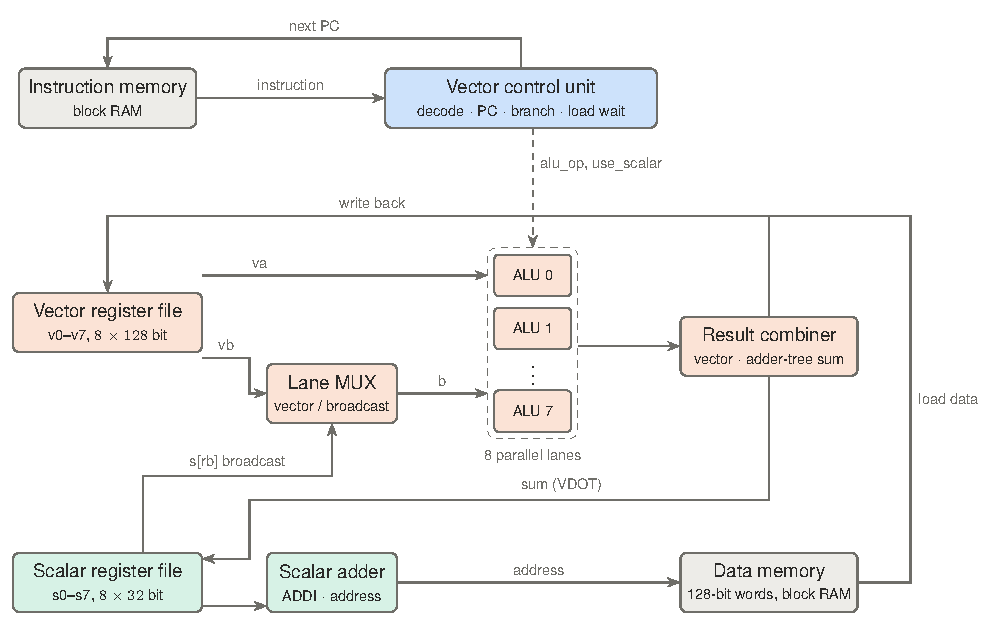
\includegraphics[width=0.86\textwidth]{figures/block_diagram.pdf}
\caption{Block diagram of the SIMD vector processing unit (8 lanes shown). Dashed: control signals.}
\label{fig:block}
\end{figure*}

\subsection{Overview}
Fig.~\ref{fig:block} shows the unit. Two parameters set its shape: the number of
lanes $L$ (1, 2, 4 or 8) and the element width $W = 16$ bits. With $L = 8$ a vector
holds $8 \times 16 = 128$ bits, the width of SSE and NEON. The instruction and data
memories sit outside the core, so the same RTL is used both in simulation and on
the FPGA (where \texttt{fpga\_top.v} adds block-RAM memories, switches and LEDs).

\subsection{Instruction set}\label{sec:isa}
Instructions are 32 bits: a 6-bit opcode, three 3-bit register fields (\texttt{rd},
\texttt{ra}, \texttt{rb}) and a signed 16-bit immediate. The two top opcode bits
select the class:
\begin{itemize}
\item \textbf{vector--vector}: $v_d[i] = v_a[i] \circ v_b[i]$ for every lane $i$;
\item \textbf{vector--scalar}: $v_d[i] = v_a[i] \circ s_b$, the scalar broadcast to all lanes;
\item \textbf{reduce}: $s_d = \sum_i (v_a[i] \circ v_b[i])$. With $\circ = \times$ this is \texttt{VDOT};
\item \textbf{memory and control}: \texttt{VLD}, \texttt{VST}, \texttt{ADDI}, \texttt{ADD}, \texttt{BNE}, \texttt{HALT}.
\end{itemize}
The operation $\circ$ is one of 14 ALU jobs: \texttt{ADD}, \texttt{SUB},
\texttt{AND}, \texttt{OR}, \texttt{XOR}, three shifts, \texttt{MUL} (low half),
\texttt{SEQ}, \texttt{SLT}, \texttt{SLTU}, \texttt{MIN} and \texttt{MAX}. Compare
jobs produce all-ones or all-zeros per lane. The vector add kernel, for example, is:
\begin{lstlisting}
      ADDI s1, s0, 0       # word index
      ADDI s2, s0, ITER    # passes = N / L
loop: VLD  v1, A(s1)
      VLD  v2, B(s1)
      VADD v3, v1, v2      # L additions at once
      VST  v3, C(s1)
      ADDI s1, s1, 1
      BNE  s1, s2, loop
      HALT
\end{lstlisting}
The same source runs on every lane count; only \texttt{ITER} changes.

\subsection{Microarchitecture}
\paragraph{Vector control unit} Decodes the instruction into control signals and
computes the next program counter. Instruction memory is synchronous (block RAM),
so the unit sends it the \emph{next} address one cycle early. Taken branches
therefore cost nothing. Loads take two cycles: the address goes out in the first,
and the returned data is written in the second.

\paragraph{Vector register file} Eight $L \cdot W$-bit registers, with two
asynchronous read ports and one synchronous write port.

\paragraph{Scalar register file (scalar interface)} Eight 32-bit registers, with
\texttt{s0} hard-wired to zero. They hold addresses, loop counters, broadcast values
and reduction results. A third, debug read port exposes any register to the host
testbench or to LEDs on the board.

\paragraph{Lane multiplexers} For each lane, operand B is either that lane's element
of $v_b$ or the low $W$ bits of $s_b$ copied to every lane.

\paragraph{Parallel ALUs} $L$ instances of a combinational 14-operation lane ALU,
created with a \texttt{generate} loop and sharing one operation code. Lanes have no
connection to each other (no carry crosses a lane boundary).

\paragraph{Result combiner} Returns the lane outputs as a vector for write-back.
It also sign-extends them to 32 bits and sums them with a $\log_2 L$-level adder tree
for the reduce instructions.

\subsection{Timing model}
Every instruction except \texttt{VLD} completes in one cycle, so a program's run time is
\begin{equation}
  \text{cycles} = \text{instructions} + \text{loads}.
\end{equation}
For a kernel with $k$ set-up instructions, a loop body of $b$ instructions with
$\ell$ loads, and $N$ elements on $L$ lanes,
\begin{equation}
  C(L) = k + \frac{N}{L}\,(b + \ell) + 1, \qquad
  S(L) = \frac{C(1)}{C(L)} \;<\; L .
\end{equation}
The speed-up $S$ approaches $L$ as $N$ grows; the $k + 1$ serial instructions are
the Amdahl term.

\subsection{Verification methodology}\label{sec:verif}
Verification works in layers:
\begin{enumerate}
\item \textbf{Unit testbenches} drive each block with corner cases and seeded random
      stimulus and compare against reference models written independently of the RTL
      (for example, shifts as multiplication or division by $2^n$). The ALU test
      performs 225,496 lane checks. It counts true and false outcomes per compare
      operation and fails on any coverage hole.
\item \textbf{Golden model.} A Python instruction-set simulator executes the
      assembled machine code and predicts the final memory, registers, instruction
      count and cycle count.
\item \textbf{System testbench.} It loads a program and data, runs the core to
      \texttt{HALT}, and compares all 1,024 data-memory words, all scalar registers
      (through the debug port) and both counters with the golden model.
\item \textbf{Program check.} The golden-model result is also compared with plain
      arithmetic (e.g.\ $C_i = A_i + B_i$), which catches errors in the programs.
\item \textbf{Directed corner tests.} Hand-built programs exercise what the
      benchmarks never do: writes to \texttt{s0}, address and PC wrap-around,
      back-to-back loads, a branch into a load, a 32-bit scalar broadcast and
      every unused op code.
\item \textbf{Board check.} The FPGA top, with its block RAM and started only by
      its power-on reset, must show the golden model's dot product on its LEDs.
\item \textbf{Mutation tests.} Deliberately injected bugs (a logical instead of
      arithmetic right shift, a mis-wired adder tree, zero- instead of
      sign-extension, a missing load stall) must make the tests fail.
\end{enumerate}
A sixth program, \texttt{isa\_test}, executes all 42 vector-ALU and reduce forms on
random 16-bit data, so every instruction is exercised on the complete core.

\subsection{Experimental setup}
The five benchmark kernels are vector add, SAXPY ($Y = aX + Y$), ReLU, threshold
(a branch-free conditional using masks) and dot product, each on $N = 256$
elements with a fixed random seed. The simulator is Icarus Verilog 13; synthesis
uses Yosys~0.70 for a Lattice ECP5 LFE5U-25F (speed grade 6), with place-and-route
in nextpnr. Each ECP5 build is placed with three seeds and the median frequency is
reported. A Yosys estimate for the Xilinx Artix-7 xc7a35t (Basys-3) is also given.

% =============================================================================
\section{Prototype Status and Preliminary Results}\label{sec:results}

\subsection{Verification}
All unit tests pass, and all 24 system runs (6 programs $\times$ 4 lane counts)
and 8 directed runs match the golden model exactly in memory contents, scalar
registers, instruction count and cycle count. The board version shows the correct
dot product for every lane count. Every injected mutation was detected. Verilator lint
(\texttt{-Wall}) reports no warnings for any module; the only two waivers mark
bits that are unused on purpose. Continuous integration
repeats the lint and tests on every change.

\subsection{Scalar versus SIMD}
Table~\ref{tab:perf} gives the cycle counts. Every count equals the prediction of
(2) exactly, and the speed-up is 1.0--1.6\% below the ideal $8\times$. The gap is
the two to four set-up instructions and \texttt{HALT}, which are not
parallelised. Fig.~\ref{fig:speedup} plots the mean over the five kernels.

\begin{table}[t]
\centering
\caption{Clock cycles for $N = 256$ elements}
\label{tab:perf}
\begin{tabular}{lrrrrr}
\toprule
Kernel & $L{=}1$ & $L{=}2$ & $L{=}4$ & $L{=}8$ & Speed-up \\
\midrule
vadd      & 2051 & 1027 & 515 & 259 & $7.92\times$ \\
saxpy     & 2308 & 1156 & 580 & 292 & $7.90\times$ \\
relu      & 1539 &  771 & 387 & 195 & $7.89\times$ \\
threshold & 2053 & 1029 & 517 & 261 & $7.87\times$ \\
dot       & 2052 & 1028 & 516 & 260 & $7.89\times$ \\
\bottomrule
\end{tabular}
\end{table}

\begin{figure}[t]
\centering
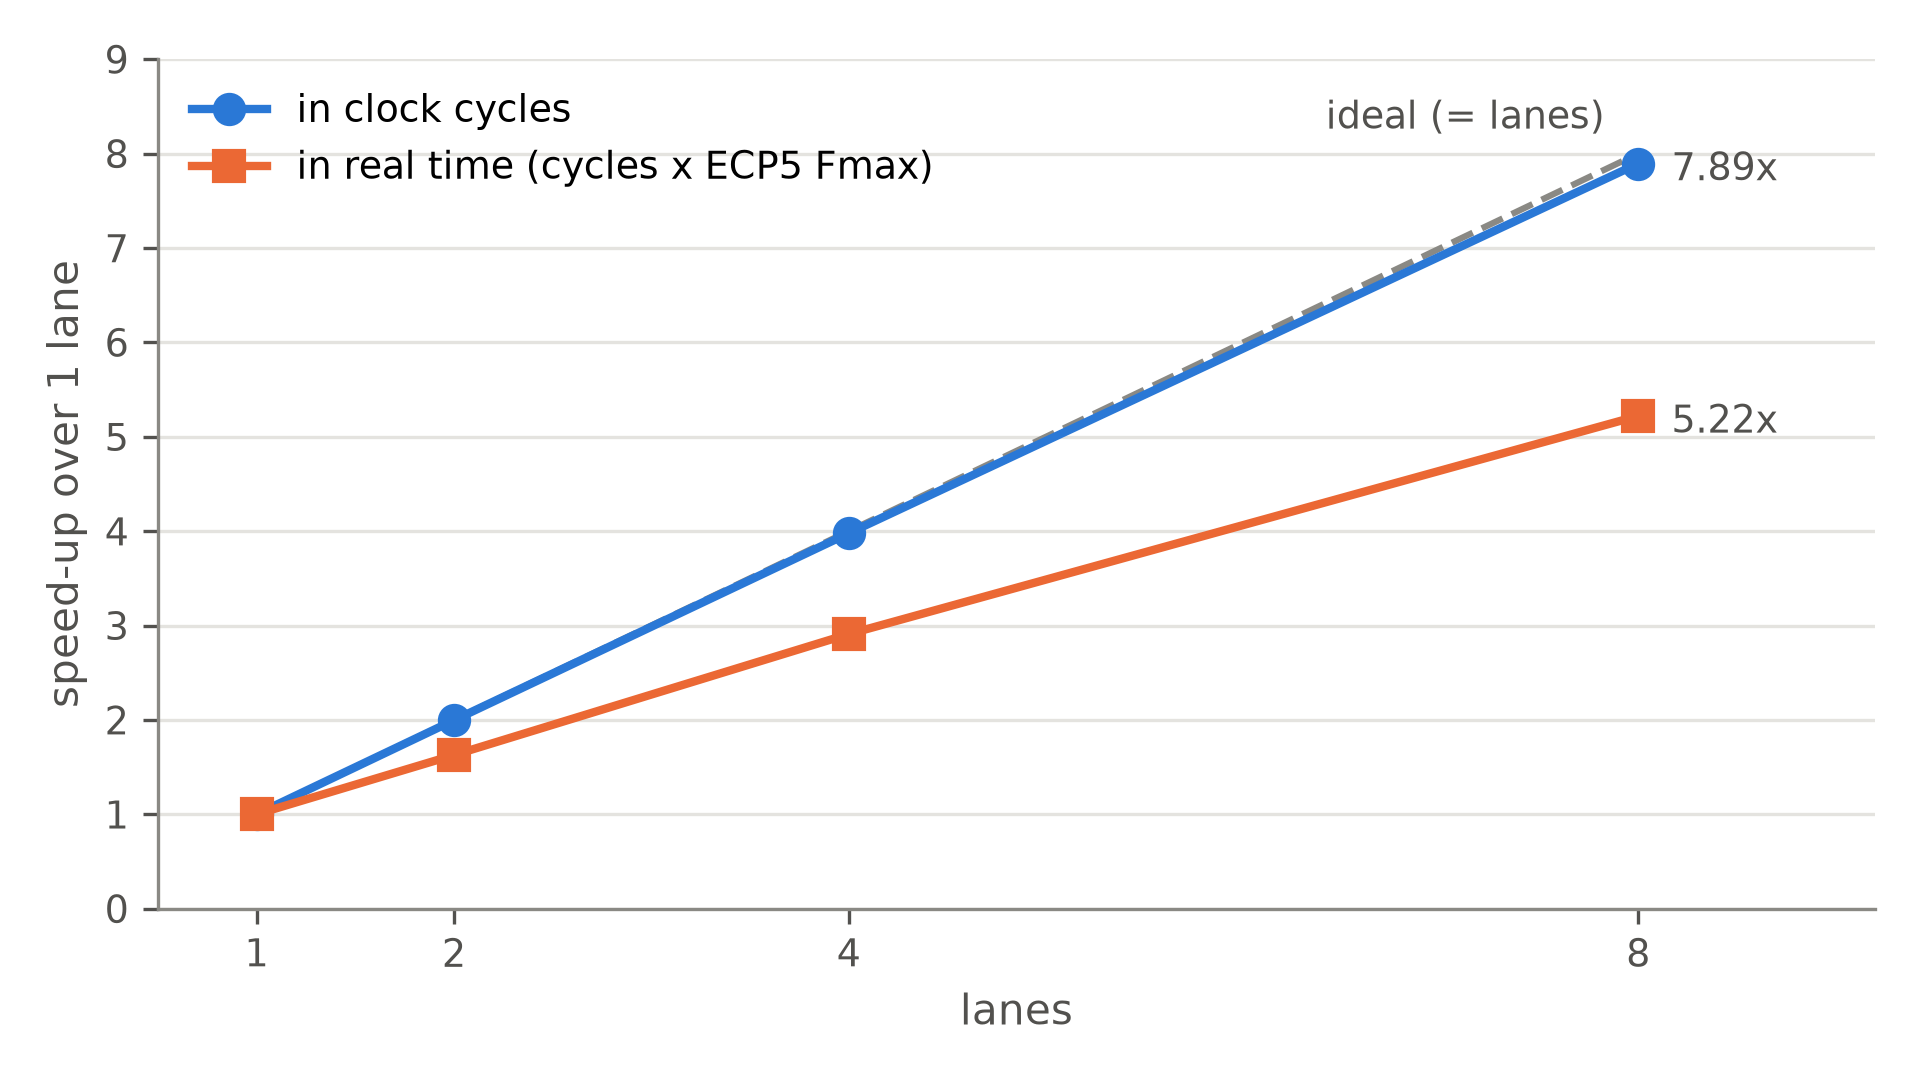
\includegraphics[width=\columnwidth]{figures/speedup.png}
\caption{Speed-up over one lane: in clock cycles (blue) and in wall-clock time once
each design's measured ECP5 $F_{\max}$ is applied (orange).}
\label{fig:speedup}
\end{figure}

\subsection{FPGA resources and frequency}
Table~\ref{tab:fpga} and Fig.~\ref{fig:fpga} summarise the ECP5 results. Each lane
adds one hardware multiplier and about 530 logic cells on average. Shared logic (control,
scalar registers, memories) is paid once, so eight lanes need $4.9\times$ the logic
of one. The register files are mapped to distributed LUT RAM, which keeps the
flip-flop count low. On the Artix-7, Yosys estimates 3,704 LUTs (18\%) and 9 DSP
slices for eight lanes.

\begin{table}[t]
\centering
\caption{Lattice ECP5-25F after place-and-route}
\label{tab:fpga}
\begin{tabular}{lrrrr}
\toprule
$L$ & Logic cells & Mult. & BRAM & $F_{\max}$ (MHz) \\
\midrule
1 &   949 \,(3.9\%)  & 1 & 2 & 50.8 \\
2 & 1,636 \,(6.7\%)  & 2 & 2 & 41.4 \\
4 & 2,865 \,(11.8\%) & 4 & 3 & 37.1 \\
8 & 4,650 \,(19.1\%) & 8 & 5 & 33.6 \\
\bottomrule
\end{tabular}
\end{table}

\begin{figure}[t]
\centering
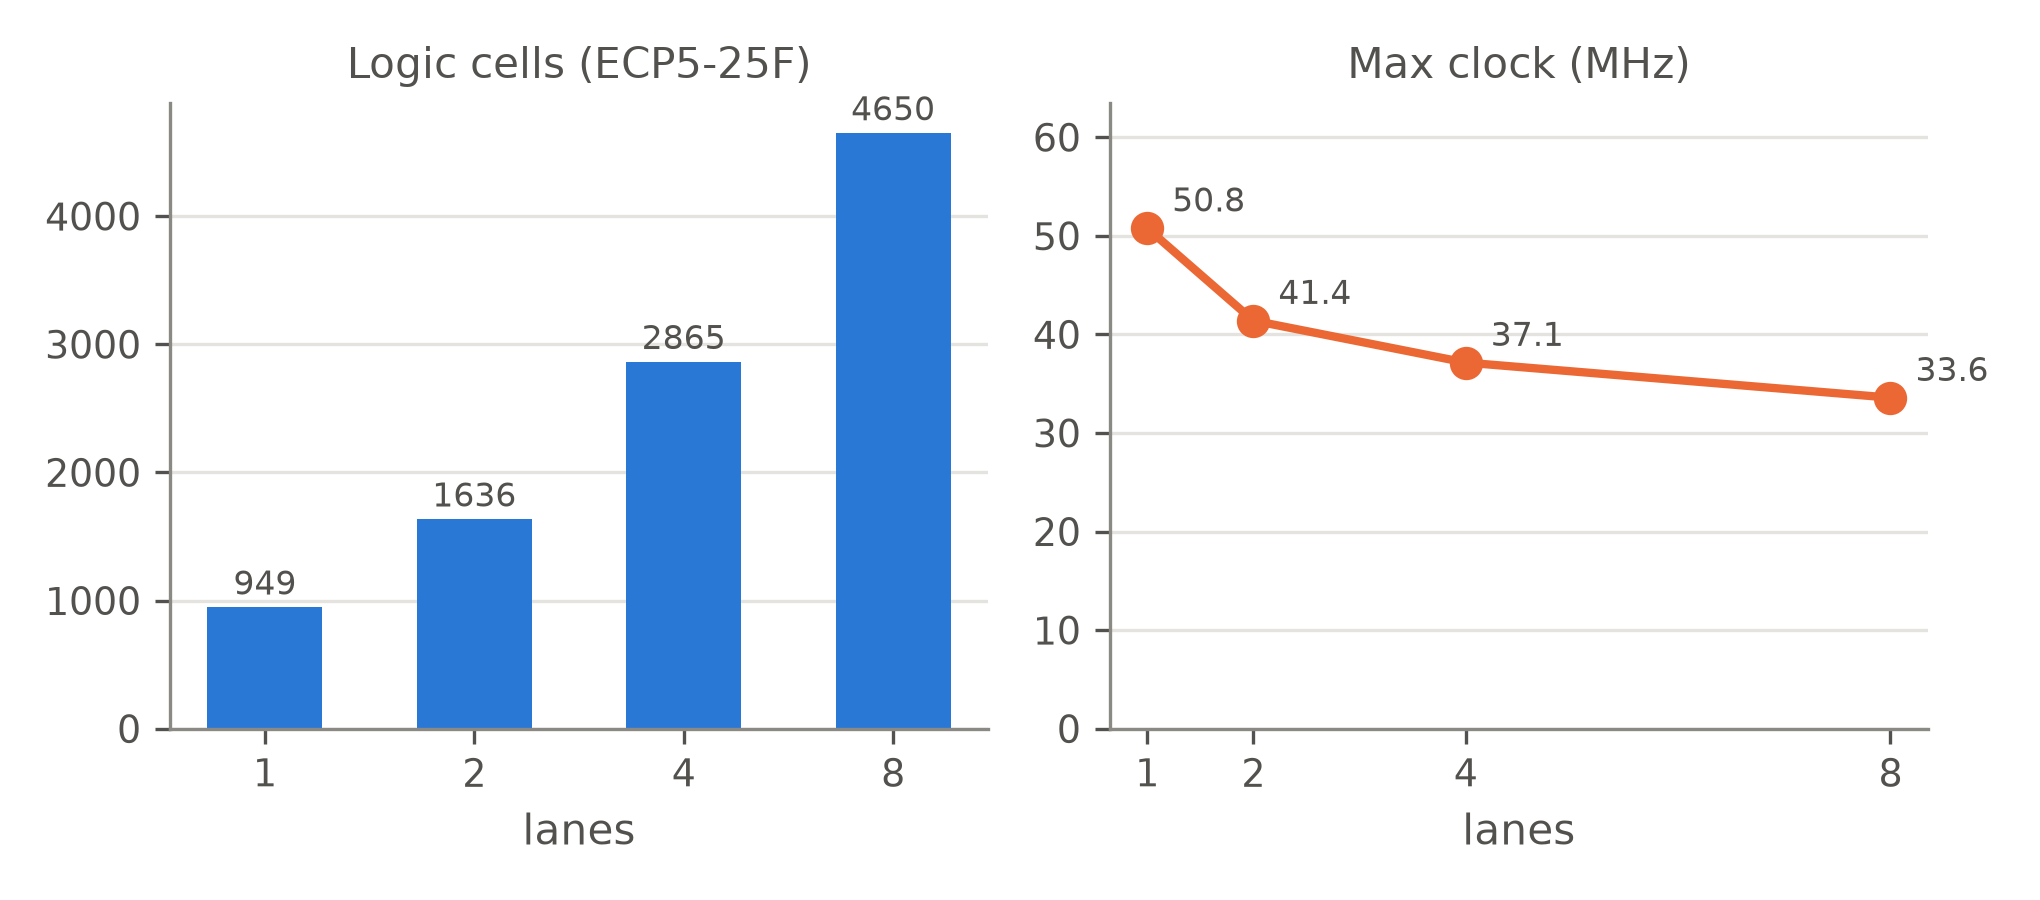
\includegraphics[width=\columnwidth]{figures/fpga_scaling.png}
\caption{ECP5-25F logic cells and maximum clock frequency against lane count
(median of three placement seeds; bars show the range).}
\label{fig:fpga}
\end{figure}

\subsection{Discussion}
The maximum frequency falls from \SI{50.8}{MHz} to \SI{33.6}{MHz} as the lanes go
from one to eight. Because the core executes each instruction in a single cycle, its
critical path crosses the whole datapath: block-RAM output, decode, register read,
multiplier, adder tree and scalar write-back. Wider designs also spread across
more of the device, which lengthens routing. The wall-clock speed-up at eight lanes
is therefore $7.89 \times 33.6/50.8 = 5.2\times$, not $7.9\times$. The result
confirms the main promise of SIMD: near-linear gains in work per instruction. It
also shows that a wider datapath must be pipelined to keep its clock rate. On a
small Lattice iCE40 UP5K (5,280 cells), the 8-lane design did not fit even with its
eight DSP blocks in use. A mid-range device is the practical minimum.

% =============================================================================
\section{Individual Contributions}

\begin{table}[h]
\centering
\caption{Work split (GitHub history shows each member's commits)}
\label{tab:contrib}
\begin{tabular}{p{0.24\columnwidth}p{0.66\columnwidth}}
\toprule
Member & Contribution \\
\midrule
Mahir (lead) & Architecture and ISA; vector control unit; core integration; instruction-level golden model and workload runner; system testbench; CI; documentation; report \\
Krishiv Gupta & Lane ALU (14 operations) and parallel ALU array; ALU testbench; FPGA wrapper and synthesis flow (ECP5 place-and-route, Artix-7, Vivado); resource and $F_{\max}$ analysis \\
Abhiman Singh & Vector and scalar register files with debug port; register-file testbench \\
Jayadeep & Lane multiplexers and result combiner (adder tree); combiner testbench for 1--8 lanes; scalar-versus-SIMD performance analysis and figures \\
Ashish Kushwaha & Assembler; the six workload programs; assembler tests \\
\bottomrule
\end{tabular}
\end{table}

\textbf{Mahir} defined the instruction format and the block interfaces that the rest
of the team built against. He wrote the vector control unit, with its early
instruction fetch and two-cycle load, and integrated the core. He wrote the
instruction-level golden model that predicts results and exact cycle counts, the
workload runner, and the system testbench that compares memory, registers and cycle
counts with the model. He also set up the repository, continuous integration and
documentation.

\textbf{Krishiv Gupta} designed the lane ALU and its \texttt{generate}-based array,
including signed and unsigned compares and arithmetic shifts. His testbench checks
225,496 lane results against an independent integer model and proves that no carry
crosses a lane boundary. He also built the FPGA wrapper and the synthesis flow that
produced the ECP5 resource and frequency results, the Artix-7 estimate, and the
Vivado script and Basys-3 constraints for the lab.

\textbf{Abhiman Singh} designed the two register files: two read ports and one
write port each, a hard-wired zero register, and the debug port that forms the
scalar interface. His testbench covers read-during-write behaviour and 4,000 random
cycles against a shadow model.

\textbf{Jayadeep} designed the lane multiplexers and the result combiner's
$\log_2 L$ adder tree, verified for every lane count. He produced the
scalar-versus-SIMD analysis: cycle counts for 1, 2, 4 and 8 lanes, speed-up,
throughput and the figures.

\textbf{Ashish Kushwaha} wrote the two-pass assembler, with labels, constants and
line-numbered error messages, and its tests. He also wrote the six workload programs,
including the branch-free threshold kernel and the instruction-coverage program.

% =============================================================================
\section{Conclusion and Phase II Plan}
The Phase~I prototype is complete and verified. An eight-lane, 128-bit SIMD unit
executes a 48-instruction ISA, matches its golden model cycle for cycle, and reaches
a $7.9\times$ cycle speed-up and a $5.2\times$ wall-clock speed-up over its own
scalar configuration on a mid-range FPGA. Phase~II will
(i)~pipeline the core to raise $F_{\max}$ and recover wall-clock speed-up;
(ii)~measure exact Artix-7 resources and timing in Vivado and run the design on a
Basys-3 board;
(iii)~add predicated (masked) execution and saturating arithmetic;
(iv)~study speed-up against problem size $N$ to quantify the Amdahl term; and
(v)~compare power estimates per operation for scalar and SIMD builds.

% =============================================================================
\begin{thebibliography}{99}

\bibitem{hp6} J.~L. Hennessy and D.~A. Patterson, \emph{Computer Architecture: A
Quantitative Approach}, 6th~ed. Cambridge, MA, USA: Morgan Kaufmann, 2017, ch.~4.

\bibitem{flynn72} M.~J. Flynn, ``Some computer organizations and their effectiveness,''
\emph{IEEE Trans. Comput.}, vol.~C-21, no.~9, pp.~948--960, Sep. 1972.

\bibitem{cray1} R.~M. Russell, ``The CRAY-1 computer system,''
\emph{Commun. ACM}, vol.~21, no.~1, pp.~63--72, Jan. 1978.

\bibitem{mmx} A.~Peleg and U.~Weiser, ``MMX technology extension to the Intel
architecture,'' \emph{IEEE Micro}, vol.~16, no.~4, pp.~42--50, Aug. 1996,
doi: 10.1109/40.526924.

\bibitem{sse} S.~K. Raman, V.~Pentkovski, and J.~Keshava, ``Implementing streaming
SIMD extensions on the Pentium III processor,'' \emph{IEEE Micro}, vol.~20, no.~4,
pp.~47--57, Jul. 2000, doi: 10.1109/40.865866.

\bibitem{viram} C.~E. Kozyrakis and D.~A. Patterson, ``Scalable vector processors
for embedded systems,'' \emph{IEEE Micro}, vol.~23, no.~6, pp.~36--45, Nov. 2003,
doi: 10.1109/MM.2003.1261385.

\bibitem{asanovic98} K.~Asanovi\'c, ``Vector microprocessors,'' Ph.D. dissertation,
Univ. California, Berkeley, CA, USA, 1998.

\bibitem{maven} Y.~Lee, R.~Avizienis, A.~Bishara, R.~Xia, D.~Lockhart, C.~Batten,
and K.~Asanovi\'c, ``Exploring the tradeoffs between programmability and efficiency
in data-parallel accelerators,'' in \emph{Proc. 38th Int. Symp. Comput. Archit.
(ISCA)}, 2011, pp.~129--140.

\bibitem{rvv} RISC-V International, ``The RISC-V `V' vector extension,''
version~1.0, 2021. [Online]. Available: \url{https://github.com/riscv/riscv-v-spec}

\bibitem{ara} M.~Cavalcante, F.~Schuiki, F.~Zaruba, M.~Schaffner, and L.~Benini,
``Ara: A 1-GHz+ scalable and energy-efficient RISC-V vector processor with
multiprecision floating-point support in 22-nm FD-SOI,'' \emph{IEEE Trans. Very
Large Scale Integr. (VLSI) Syst.}, vol.~28, no.~2, pp.~530--543, Feb. 2020.

\bibitem{intelsdm} Intel Corp., \emph{Intel 64 and IA-32 Architectures Software
Developer's Manual}, vol.~2. [Online]. Available: \url{https://www.intel.com/sdm}.
Accessed: Nov. 6, 2026.

\bibitem{armarm} Arm Ltd., \emph{Arm Architecture Reference Manual for A-profile
Architecture}. [Online]. Available: \url{https://developer.arm.com/documentation/ddi0487/latest}.
Accessed: Nov. 6, 2026.

\bibitem{msa} MIPS Technologies, ``MIPS SIMD Architecture,'' white paper, rev.~1.00, 2012.

\bibitem{vespa} P.~Yiannacouras, J.~G. Steffan, and J.~Rose, ``VESPA: Portable,
scalable, and flexible FPGA-based vector processors,'' in \emph{Proc. Int. Conf.
Compilers, Archit. Synth. Embedded Syst. (CASES)}, 2008, pp.~61--70.

\bibitem{vipers} J.~Yu, C.~Eagleston, C.~H.-Y. Chou, M.~Perreault, and G.~Lemieux,
``Vector processing as a soft processor accelerator,'' \emph{ACM Trans.
Reconfigurable Technol. Syst.}, vol.~2, no.~2, pp.~12:1--12:34, 2009,
doi: 10.1145/1534916.1534922.

\bibitem{vegas} C.~H. Chou, A.~Severance, A.~D. Brant, Z.~Liu, S.~Sant, and
G.~G.~F. Lemieux, ``VEGAS: Soft vector processor with scratchpad memory,'' in
\emph{Proc. ACM/SIGDA Int. Symp. Field Program. Gate Arrays (FPGA)}, 2011,
pp.~15--24.

\bibitem{mxp} A.~Severance and G.~G.~F. Lemieux, ``Embedded supercomputing in
FPGAs with the VectorBlox MXP matrix processor,'' in \emph{Proc. Int. Conf.
Hardware/Software Codesign Syst. Synth. (CODES+ISSS)}, 2013, pp.~1--10,
doi: 10.1109/CODES-ISSS.2013.6658993.

\bibitem{amdahl} G.~M. Amdahl, ``Validity of the single processor approach to
achieving large scale computing capabilities,'' in \emph{Proc. AFIPS Spring Joint
Comput. Conf.}, 1967, pp.~483--485.

\bibitem{nextpnr} D.~Shah, E.~Hung, C.~Wolf, S.~Bazanski, D.~Gisselquist, and
M.~Milanovi\'c, ``Yosys+nextpnr: An open source framework from Verilog to bitstream
for commercial FPGAs,'' in \emph{Proc. IEEE 27th Annu. Int. Symp.
Field-Program. Custom Comput. Mach. (FCCM)}, 2019, arXiv:1903.10407.

\bibitem{icarus} S.~Williams, ``Icarus Verilog,'' 2026. [Online]. Available:
\url{https://steveicarus.github.io/iverilog/}

\end{thebibliography}

\end{document}
